
\section{Theorie}
\label{sec:Theorie}


Für die magnetische Flussdichte eines Magnetfeldes gilt in Materie:
\begin{equation}
\vec{B}=\mu_0 \vec{H}+\vec{M}\text{,}
\end{equation}
wobei $\vec{H}$ die magnetische Feldstärke, $\mu_0$ die magnetische Feldkonstante und $\vec{M}$ die Magnetisierung des Materials ist. Sie kommt durch die Summe der atomaren magnetischen Momente pro Volumen in der Materie zustande. Die Magnetisierung steht gegebenenfalls im direktem Zusammenhang mit der anliegenden magnetischen Feldstärke. Es gilt:
\begin{equation}
	\vec{M}=\mu_0 \sum\limits_{i} \vec{u}_i = \mu_0 N \bar{\vec{u}} =\mu_0 \chi \vec{H}
\end{equation}
mit der Suszeptibilität $\chi$. Diese ist materialspezifisch und hängt insbesondere von der magnetischen Feldstärke und auch von der Temperatur ab. Es wird zwischen verschiedenen Arten des Magnetismus unterschieden. Eine ist der Paramagnetismus. Der Paramagnetismus kommt durch die Ausrichtung der magnetischen Momente, die jeweils von Drehimpulsen abhängen, zu einem magnetischen Feld zustande. Der Gesamtdrehimpuls $\vec{J}$ kann in drei Anteile aufgeteilt werden: dem Bahndrehimpuls der Elektronenhülle $\vec{L}$, dem Eigendrehimpuls der Elektronen $\vec{S}$ und dem Kerndrehimpuls. Der Kerndrehimpuls hat jedoch keinen großen Einfluss auf das magnetische Moment. Für die magnetischen Momente gilt:
\begin{equation}
	\vec{u}_\text{L}=-\frac{\mu_\text{B}}{\hslash} \vec{L}
\end{equation}
\begin{equation}
	\vec{u}_\text{S}=-g_\text{S} \frac{\mu_\text{B}}{\hslash} \vec{S}
\end{equation}
\begin{equation}
	\mu_\text{B}=\frac{e_0}{2 m_0} \hslash \text{,}\label{eq:muB}
\end{equation}
\begin{figure}
	\centering
	\caption{Ein Vektordiagramm der Drehimpulse und der magnetischen Momente.}
	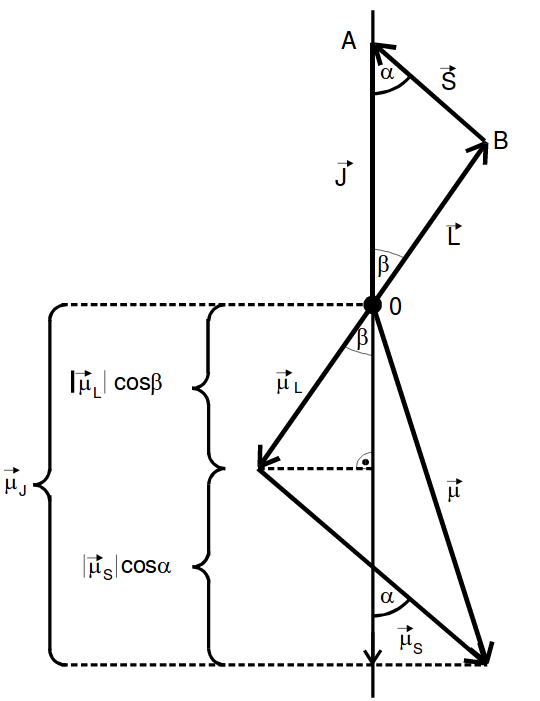
\includegraphics[width=\linewidth-70pt,height=\textwidth-200pt,keepaspectratio]{content/images/Vektordiagramm.png}
	\label{fig:Vektordiagramm}
\end{figure}
wobei $\mu_\text{B}$ das Bohrsche Magneton und $g_\text{S}$ das gyromagnetische Verhältnis des freien Elektrons ist. Die Drehimpulse sind gequantelt und es gilt für jeden der Drehimpulse $|\vec{A}|= \sqrt{A(A+1)} \hslash$. Durch Einsetzen, Umformen mithilfe der in Abbildung \ref{fig:Vektordiagramm} dargestellten Relationen und der Näherung $g_\text{S}\approx 2$ ergibt sich schließlich für den Betrag des gesamten Drehmomentes:
\begin{equation}
	|\vec{u}_\text{J}|\approx \mu_\text{B} g_\text{J} \sqrt{J(J+1)} \text{.}
\end{equation}
Der Landé-Faktor $g_\text{J}$ lässt sich folgendermaßen berechnen:
\begin{equation}
	g_\text{J}=\frac{3 J(J+1) + \{S(S+1) - L(L)\}}{2 J(J+1)}\text{.}\label{eq:g_J}
\end{equation}
Nun ist auch die Richtung des magnetischen Momentes gequantelt. Es gibt $2 J +1$ verschiedene Winkel zwischen dem magnetischem Moment und dem anliegenden magnetischen Flusses, welche die jeweilige potentielle Energie bestimmen. Nun kann die Besetzungshäufigkeit eines Energieniveaus in Abhängigkeit von der Temperatur durch die Boltzmann-Verteilung beschrieben werden. Dadurch kann das mittlere magnetische Moment bestimmt werden:
\begin{equation}
	\bar{u}\approx -\mu_\text{B} g_\text{J} \frac{\sum\limits_{m=-J}^{J} m \exp\left(\frac{-\mu_\text{B} g_\text{J} m B}{k T}\right)}{\sum\limits_{m=-J}^{J} \exp\left(\frac{-\mu_\text{B} g_\text{J} m B}{k T}\right)}\text{.}
\end{equation}
Hierin bezeichnet $B$ den Betrag des magnetischen Flusses, $k$ die Boltzmann-Konstante und $T$ die Temperatur.  Durch eine Näherung für Zimmertemperatur und Feldern unter $\SI{1}{\tesla}$ folgt für die gesuchte paramagnetische Suszeptibilität
\begin{equation}
	\chi \approx \frac{\mu_0 \mu_\text{B}^2 g_\text{J}^2 N J(J+1)}{3 k T}\text{.}\label{eq:chitheo}
\end{equation}


\subsection{Berechnung der Suszeptibilität von Seltenen-Erd-Verbindungen}
Um nun für verschiedene Materialien die magnetische Suszeptibilität berechnen zu können sind Kenntnisse über die Bahnimpulsquantenzahl $L$, die Spinquantenzahl $S$ und die Gesamtdrehimpulsquantenzahl $J$ des Materials notwendig. Bei seltenen Erden tragen nur die Elektronen in der $4f$-Unterschale zu diesen bei. Es ist also notwendig die Anzahl der Elektronen in dieser Unterschale zu kennen. Die Anordnung der Elektronen und der daraus resultierenden Drehimpulse können mit den folgenden Hundschen Regeln bestimmt werden:
\begin{enumerate}
	\item Der Gesamtspin $S=\sum\limits_{i} s_i$ ist maximal unter Berücksichtigung des Pauli-Prinzips. \label{Regel1}
	\item Der Gesamtbahndrehimpuls $L=\sum\limits_i l_i$ ist unter Berücksichtigung von Regel \ref{Regel1} und dem Pauli-Prinzip maximal. \label{Regel2}
	\item Der Gesamtdrehimpuls ist $J=L+S$ falls die Anzahl der Elektronen in der Schale großer als die Hälfte der maximal möglichen Anzahl ist, ansonsten $J=L-S$. \label{Regel3}
\end{enumerate}
In einer $4f$-Schale ist ein maximaler Bahndrehimpuls $l$ von 3 und ein Spin $s$ von $\pm \frac{1}{2}$ möglich. Da nach dem Pauli-Prinzip nur jeweils ein Elektron die gleiche Kombination von Bahndrehimpuls und Spin haben kann, können in der $4f$-Unterschale bei Seltenen-Erd-Atomen maximal 14 Elektronen vorkommen.